\documentclass[conference]{IEEEtran}
%\IEEEoverridecommandlockouts
% The preceding line is only needed to identify funding in the first footnote. If that is unneeded, please comment it out.
\usepackage{cite}
\usepackage{amsmath,amssymb,amsfonts}
\usepackage{algorithmic}
\usepackage{graphicx}
\usepackage{textcomp}
\usepackage{xcolor}
\def\BibTeX{{\rm B\kern-.05em{\sc i\kern-.025em b}\kern-.08em
    T\kern-.1667em\lower.7ex\hbox{E}\kern-.125emX}}
\begin{document}

\title{Commitment Schemes}

\author{Leonhard Applis}

\maketitle

\begin{abstract}
This Paper summarizes and  introduces to  the topic of Commitment-Schemes, a two party kryptographic protocol. 

The aim of commitment schemes is to provide a mechanism for Party A to commit to a hidden value and reveal it if necessary. Party B can confirm that the revealed value and the hidden value match.

~\newline This Paper first introduces to the topic itself, a hash-based implementation and the \textit{pedersen-commitments} which are based on the discrete logarithm. In Conclusion a Case-study of commitments for one-time authorization in a distributed web-application is provided. 
\end{abstract}

\section{Introduction}
The Internet is a land of mistrust - for good reasons. Yet it is often required to trust each other. 

\subsection{Protocol}
The following steps are considered the basic protocol of commitment-schemes and vary only in their implementation. Often the protocol is shortened to only two steps, the commitment and the reveal (step 1 and 3), as these are the only steps requiring communication. This shortened version is also depicted in figure \ref{fig:protocoll}.  
\begin{enumerate}
	\item A \textbf{commits} to B
	\item B keeps commitment, unable to read or process it
	\item A \textbf{reveals} to B
	\item B verifies the commitment 
\end{enumerate}

\begin{figure}
	\centering
	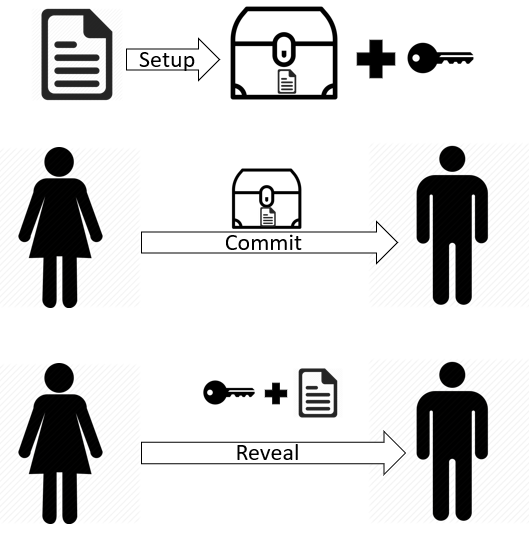
\includegraphics[width=0.8\linewidth]{Images/protocoll}
	\caption[Commitments]{Commitments}
	\label{fig:protocoll}
\end{figure}

\subsection{Attributes}
The following attributes are required for commitment-schemes to be secure and successfully fulfill their purpose.

\begin{enumerate}
	\item \textbf{Binding:} The values Alice put in the commitment cannot be changed after Bob recieved it 
	\item \textbf{Hiding:} Bob cannot gain any information about the message from the commitment itself
	\item \textbf{Viability:} If both parties follow the protocol correct, Bob is always able to recover the committed value
\end{enumerate}
Except for viability, the fulfillment of each attribute will be shortly discussed in the regarding implementations. 

There are two additional attributes based on the fact that we are working with computers:
\begin{enumerate}
	\item Bobs are able compare commitments.
	\item Commitments are \textit{tradeable} and replicable - both for Alice and Bob, still keeping their primary attributes and are fully functional. This attribute is vital for the case study presented in section \ref{sec:casestudy}.
\end{enumerate}


\subsection{Additional Security-Measures}
There are several \textit{best-practices} which are not functional for the protocol itself, but are necessary to secure any party involved in the protocol and any application using the protocols. They will be shortly summarized and explained: ~\newline

	\paragraph{commitments should be one- (positive-) use only} This originates from the \textit{reveal}-step, in which everything required to reveal the commitment successfully is transmitted. An eavesdropper would after the initial reveal be able to copy the required \textit{credentials} and also reveal the commitment correct.  To fix this issue, simply mark used commitments as deprecated (if they are further required), or delete them completely. 
	\paragraph{commitments should have a lifetime} (in time and/or tries)
	This behavior helps against brute-force attacks from exterior, given that the attacking party does not hold the commitment itself. If an aggressor has the commitment, he can start brute-force attacks locally (this holds true for eve and bob) which still requires \textbf{safe} cryptographic implementations.
	Additionally the lifetime (in e.g. days) is useful for Bob, as he has limited resources and should only keep \textit{required} information. 
	\paragraph{traded commitments to a third party should be deprecated directly with first reveal} This is an extended version of the problem shown in paragraph \textit{a)} of this subsection. Given there are multiple copies of the same commitment, and an eavesdropper knows the parties which hold a copy, Eve can successfully reveal the commitment to any party. For addressing this issue, the commitments need to be recursively deprecated throughout any party which the commitment was shared to. A common way to do this for Bob is to reveal the commitment by himself - this method does not require additional structures and also verifies that Bob knows the correct values. 
	
	However, if there is a larger number of parties involved, Eve can be \textit{faster} reaching to the last Bob and reveal the commitment. Additionally there are many attacks that disturb the communication between Bob's, thus leaving more chances for Eve to reveal herself as Alice. Sharing commitments should be therefore only used when required. 
	\paragraph{messages must contain random parts} This rather trivial point is important for any implementation to fulfill any attribute connected to the \textit{computational safeness} of hashfunctions and the discrete logarithm.  
~\newline ~\newline
For every implementation based on commitment-schemes all of the above should be taken to account. There are several problems if only a single point is left out, including identity theft and server-malfunctions. 

There are common libraries which support you in the goal of a secure implementation, e.g. an implementation in Haskell \cite{b0} . The use of an open-source and \textbf{maintained} library is highly recommended.
\section{Implementation}

\subsection{Hash-Based Commitments}
ToDo: Hash-Based Commitments with sources
	
	\begin{enumerate}
		\item Alice chooses a random value $s$
		\item Alice produces $h = Hash(m \star s)$ and sends $h$ and $Hash$ to Bob
		\item Bob keeps $<Alice,h,Hash>$
		\item Alice reveals herself by sending bob $m$ and $s$
		\item Bob checks if $Hash(m \star s) \equiv h$
	\end{enumerate}

\subsection{Pedersen Commitments}
ToDo: Pedersen Commitments with sources
SetUp:
	\begin{enumerate}
		\item choosing a large prime number p
		\item choosing a smaller prime number $q \in \{1..p| q\div (p-1) = 0\}$
		\item choosing $g,v \in G_q \neq 1$
		\item sending Alice $p,q,g,v$ 
	\end{enumerate}
Protocoll: 
	\begin{enumerate}
		\item Alice requests $p,q,g,v$ from Bob. \newline Alice checks that:
		\begin{itemize}
			\item $q,p$ are primes, 
			\item q divides p-1, 
			\item that $g,v \in G_q$. 
		\end{itemize}
		\item Alice chooses her message $m \in \{1..p\}$ and a random number $r \in \{1..q-1\}$
		\item Alice sends $c = g^rv^m$ to Bob \textbf{(commit)}
		\item Bob keeps $<Alice,c,<p,q,g,v>>$
		\item Alice can reveal herself by sending $r,m$ to Bob. ~\newline Bob checks $c = g^rv^m$
	\end{enumerate}

\subsection{Quadratic-Residues}
Iff i need more content

\section{Case-Study: Migrating user privileges in web-applications}
\label{sec:casestudy}.
ToDo: Describe Web-Application, Requirements and the Solution

\section*{References}

Please number citations consecutively within brackets \cite{b1}. The 
sentence punctuation follows the bracket \cite{b2}. Refer simply to the reference 
number, as in \cite{b3}---do not use ``Ref. \cite{b3}'' or ``reference \cite{b3}'' except at 
the beginning of a sentence: ``Reference \cite{b3} was the first $\ldots$''

Number footnotes separately in superscripts. Place the actual footnote at 
the bottom of the column in which it was cited. Do not put footnotes in the 
abstract or reference list. Use letters for table footnotes.

Unless there are six authors or more give all authors' names; do not use 
``et al.''. Papers that have not been published, even if they have been 
submitted for publication, should be cited as ``unpublished'' \cite{b4}. Papers 
that have been accepted for publication should be cited as ``in press'' \cite{b5}. 
Capitalize only the first word in a paper title, except for proper nouns and 
element symbols.

For papers published in translation journals, please give the English 
citation first, followed by the original foreign-language citation \cite{b6}.

\begin{thebibliography}{00}
	\bibitem[HaHa]{b0} Pederson Commitment Schemes - a Haskell Library url: http://hackage.haskell.org/package/pedersen-commitment 
	last seen: 29 Dezember 2018
	maintained at the Massachusets Institute for Technology
\bibitem{b1} G. Eason, B. Noble, and I. N. Sneddon, ``On certain integrals of Lipschitz-Hankel type involving products of Bessel functions,'' Phil. Trans. Roy. Soc. London, vol. A247, pp. 529--551, April 1955.
\bibitem{b2} J. Clerk Maxwell, A Treatise on Electricity and Magnetism, 3rd ed., vol. 2. Oxford: Clarendon, 1892, pp.68--73.
\bibitem{b3} I. S. Jacobs and C. P. Bean, ``Fine particles, thin films and exchange anisotropy,'' in Magnetism, vol. III, G. T. Rado and H. Suhl, Eds. New York: Academic, 1963, pp. 271--350.
\bibitem{b4} K. Elissa, ``Title of paper if known,'' unpublished.
\bibitem{b5} R. Nicole, ``Title of paper with only first word capitalized,'' J. Name Stand. Abbrev., in press.
\bibitem{b6} Y. Yorozu, M. Hirano, K. Oka, and Y. Tagawa, ``Electron spectroscopy studies on magneto-optical media and plastic substrate interface,'' IEEE Transl. J. Magn. Japan, vol. 2, pp. 740--741, August 1987 [Digests 9th Annual Conf. Magnetics Japan, p. 301, 1982].
\bibitem{b7} M. Young, The Technical Writer's Handbook. Mill Valley, CA: University Science, 1989.
\end{thebibliography}
\vspace{12pt}
\end{document}
